\vspace{-0.5cm}
\section*{Generell}
	\begin{minipage}[t]{12.5cm}
		\subsection*{Datentypen}
			\rowcolors{1}{blue!10}{white}
			\begin{tabular}{|>{\bfseries}l l l|}
				\hline Datentyp & \bfseries{Beschreibung} & \bfseries{False-Wert}
				\\\hline NoneType & Indikator für nichts & None
				\\\hline \multicolumn{3}{|l|}{\bfseries{Numerische Datentypen}}
				\\ int & Ganze Zahlen & 0
				\\ float & Gleitkommazahlen & 0.0
				\\ bool & Boolesche Werte & False
				\\ complex & Komplexe Zahlen & 0 + 0j
				\\\hline \multicolumn{3}{|l|}{\bfseries{Sequenzielle Datentypen}}
				\\ str & Zeichenketten oder Strings(unveränderlich) & ' '
				\\ list & Listen(veränderlich) & []
				\\ tuple & Tupel(unveränderlich) & ()
				\\ bytes & Sequenz von Bytes(unveränderlich) & b' '
				\\ bytesarray & Sequenz von Bytes(veränderlich) & bytearray(b' ')
				\\\hline Mengen & & 
				\\ set & Einmalig vorkommende Objekte & set()
				\\ frozenset & Wie set jedoch unveränderlich & frozenset()
				\\\hline \multicolumn{3}{|l|}{\bfseries{Assoziative Datentypen}}
				\\ dict & Dictionary(veränderlich) & { }
				\\\hline
			\end{tabular}
	\end{minipage}
		%\hspace*{1cm}
		\begin{minipage}[t]{3cm}
			%\vspace*{0.7cm}
			\subsection*{Operatoren}
				\rowcolors{1}{blue!10}{white}
				\begin{tabular}{|l l|}
					\hline \bfseries{Operator} & \bfseries{Beschreibung} \\\hline
					x // y & Ganzzahliger Quotient\\
					x ** y & Potenzieren, $x^y$ \\ 
					+,-,... & Übliche Operation\\\hline
				\end{tabular}
			\subsection*{Variablen}
				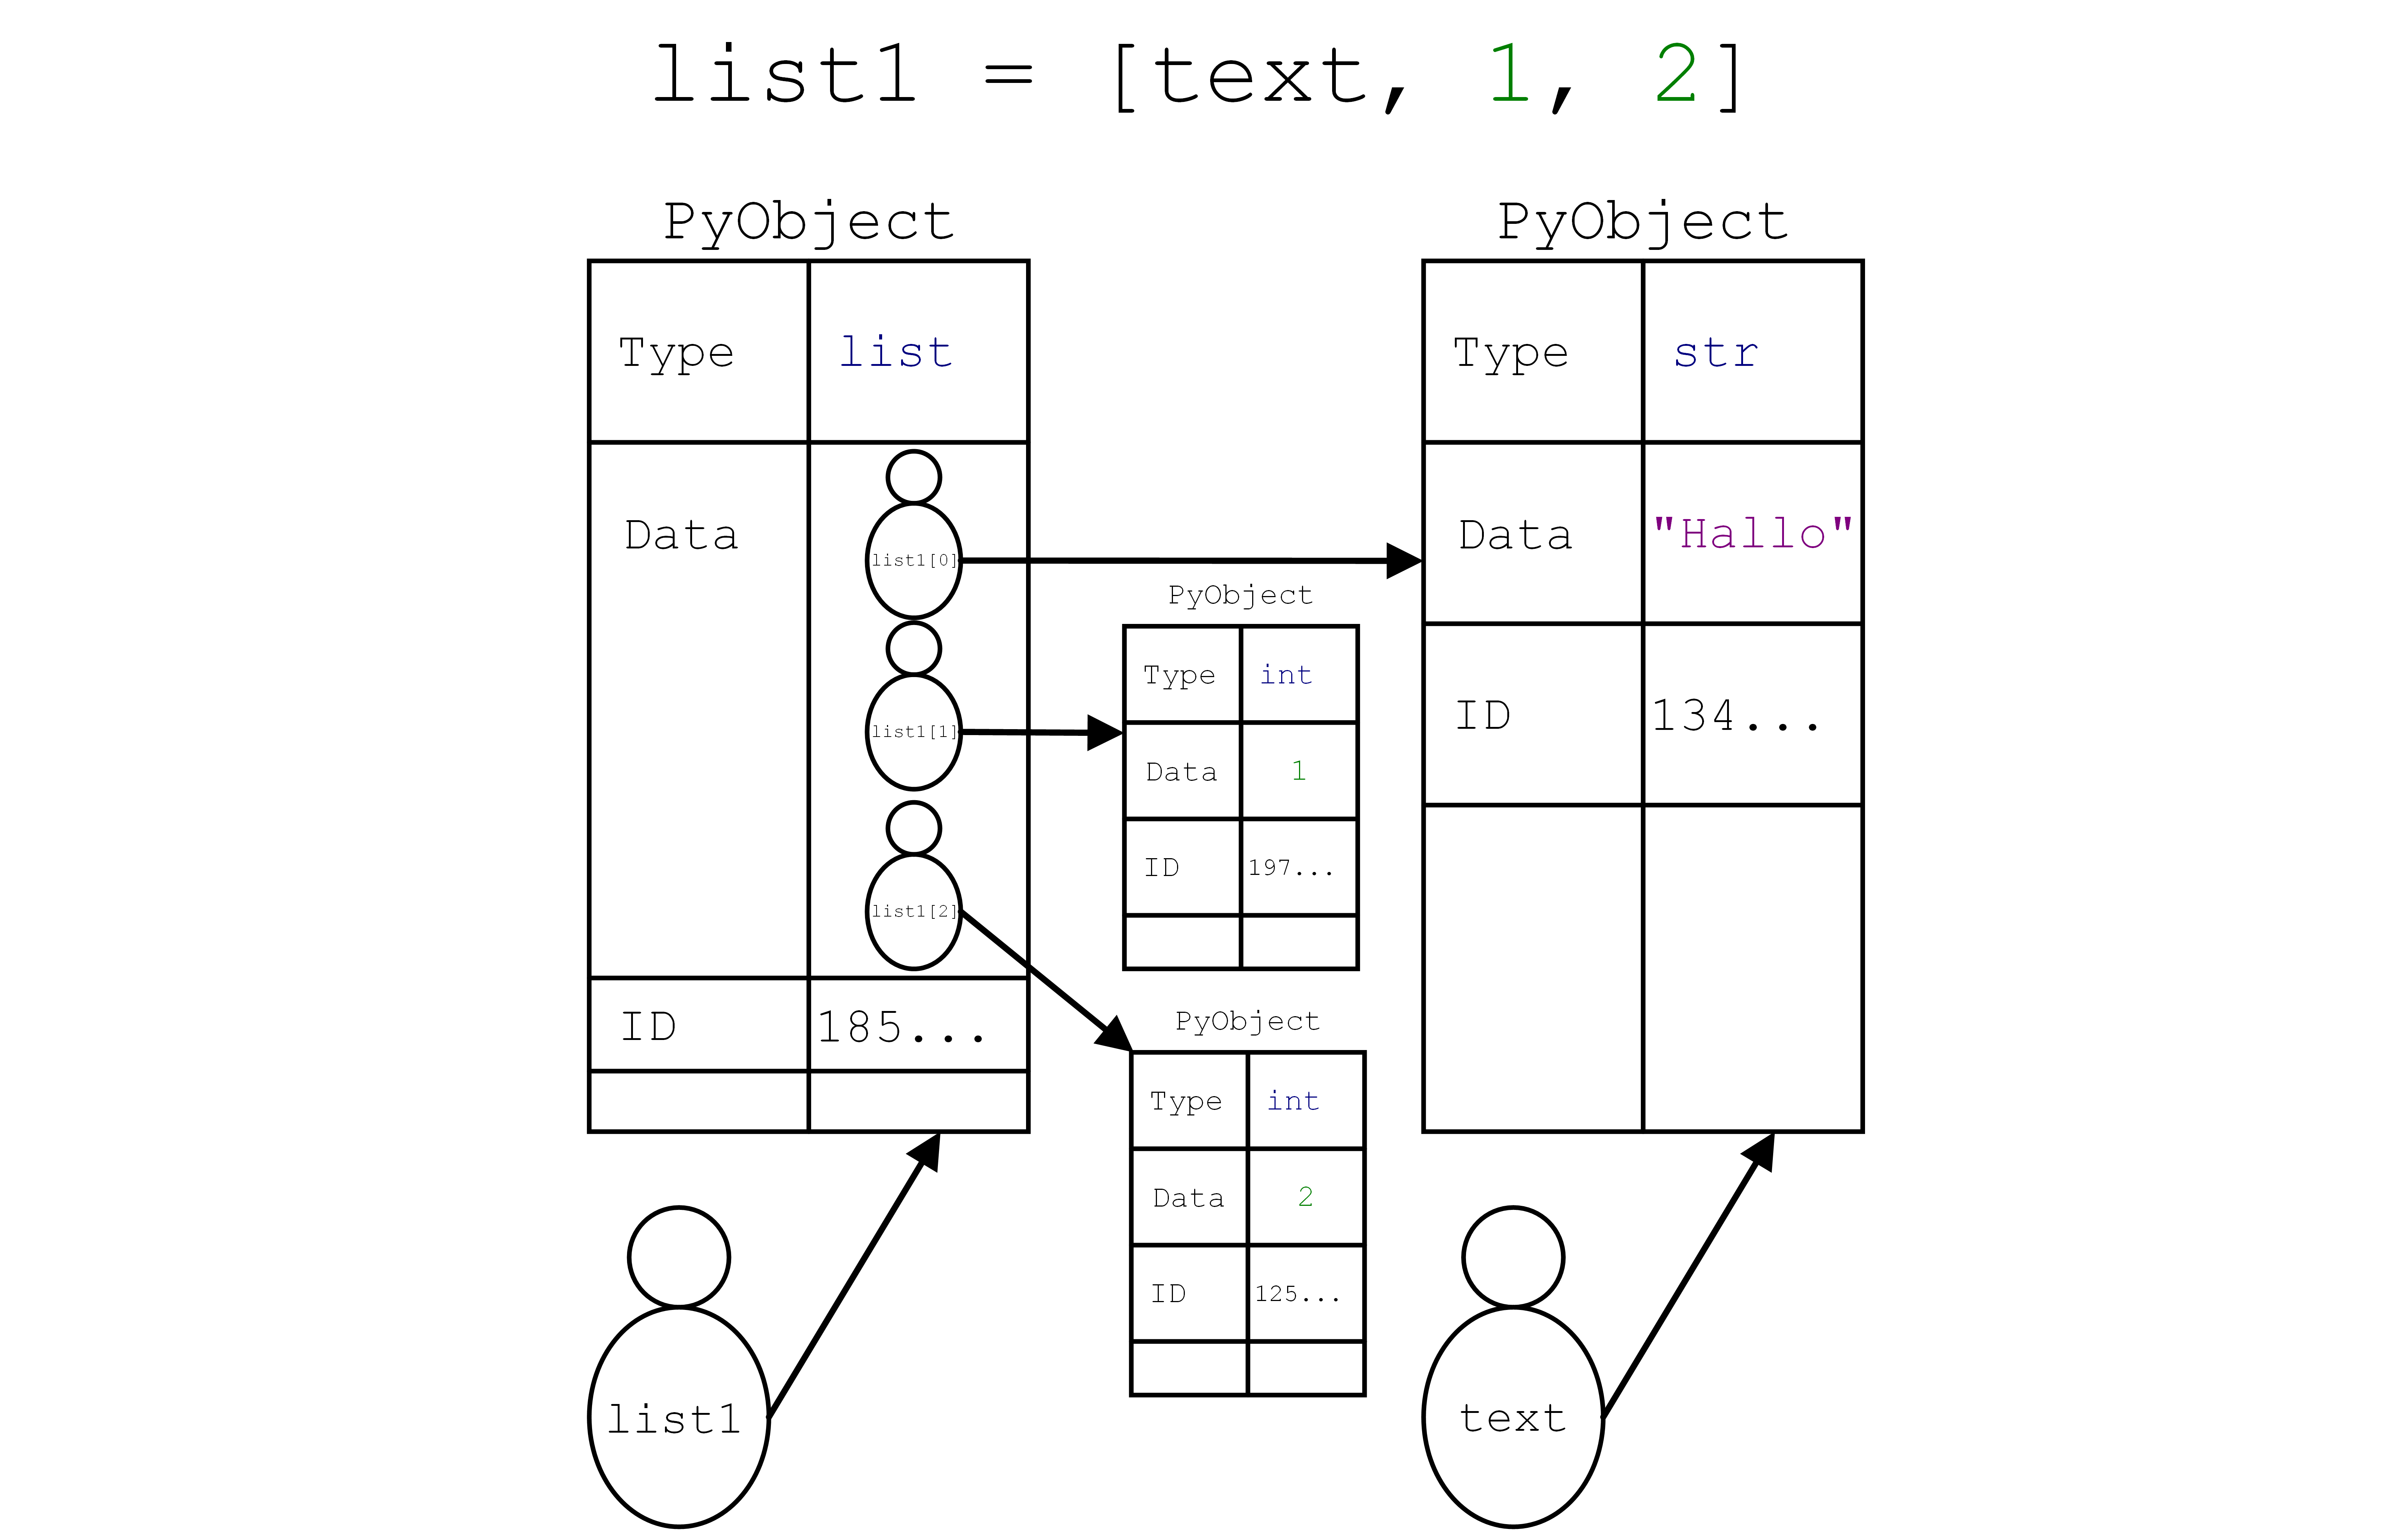
\includegraphics[height=4.5cm, align=t]{pics/Variablen.PNG}
		\end{minipage}
	\subsection*{Numerische Datentypen}
	Die numerischen Datentypen sind gleichermaßen zu behandeln wie in den bekannten Programmiersprachen.
	\subsection*{Sequenzielle Datentypen}
	\subsection{Strings}
	\lstinputlisting{code/Strings.py}